\section{Method}

%------------------------------------------------------------------------------
\begin{figure*}[t]
\centering
% editable at https://docs.google.com/drawings/d/1nfqVV_dNqSV9g5UBuNopPLvubcEZx-vvg4K0ZCvNdfU/edit
\fig[.7]{CA-CAM}
\vspace{3pt}
\caption{\emph{Visualization of eq.~\eq{connection}.} On the left, a feature tensor $\vF \in \real^{w \times h \times d}$ is multiplied by the vector $\valpha \in \real^d$ in the channel dimension, like in $1 \times 1$ convolution, where $w \times h$ is the spatial resolution and $d$ is the number of channels. This is \emph{cross attention} (CA)~\cite{dosovitskiy2020image} between the query $\valpha$ and the key $\vF$. On the right, a linear combination of feature maps $F^1, \dots, F^d \in \real^{w \times h}$ is taken with weights $\alpha_1, \dots, \alpha_d$. This is a \emph{class activation mapping} (CAM)~\cite{zhou2016learning} with class agnostic weights. Eq.~\eq{connection} expresses the fact that these two quantities are the same, provided that $\valpha = (\alpha_1, \dots, \alpha_d)$ and $\vF$ is reshaped as $F = (\vf^1 \dots \vf^d) \in \real^{p \times d}$, where $p = wh$ and $\vf^k = \vect(F^k) \in \real^{p}$ is the vectorized feature map of channel $k$.}
\label{fig:connection}
\end{figure*}
%------------------------------------------------------------------------------

\subsection{Preliminaries and background}
\label{subsec:prelim}

\paragraph{Notation}

Let $f: \cX \rightarrow \real^C$ be a classifier network that maps an input image $\vx \in \cX$ to a logit vector $\vy= f(\vx) \in \real^C$, where $\cX$ is the image space and $C$ is the number of classes. A class probability vector is obtained by $\vp = \softmax(\vy)$. The logit and probability of class $c$ are respectively denoted by $y^c$ and $p^c = \softmax(\vy)^c \defn e^{y^c} / \sum_j e^{y^j}$. Let $\vF_\ell \in \real^{w_\ell \times h_\ell \times d_\ell}$ be the feature tensor at layer $\ell$ of the network, where $w_\ell \times h_\ell$ is the spatial resolution and $d_\ell$ the embedding dimension, or number of channels. The feature map of channel $k$ is denoted by $F^k_\ell \in \real^{w_\ell \times h_\ell}$. By $\ell$ we may refer to an arbitrary layer of $f$ or a larger compositional block, \eg, a stage.

\paragraph{CAM-based saliency maps}

Given a class of interest $c$ and a layer $\ell$, we consider the saliency maps $S^c_\ell \in \real^{w_\ell \times h_\ell}$ given by the general formula
\begin{equation}
	S^c_\ell \defn h \left( \sum_k \alpha^c_k F^k_\ell \right),
\label{eq:sal}
\end{equation}
where $\alpha^c_k$ are weights defining a linear combination over channels and $h$ is an activation function. Assuming \emph{global average pooling} (GAP) of the last feature tensor $\vF_L$ followed by a linear classifier, CAM~\citep{zhou2016learning} is defined for the last layer $L$ only, with $h$ being the identity mapping and $\alpha^c_k$ the classifier weight connecting channel $k$ with class $c$. Grad-CAM~\citep{DBLP:journals/corr/SelvarajuDVCPB16} is a generalization of CAM defined for any architecture and layer $\ell$, with $h = \relu$ and weights
\begin{equation}
	\alpha^c_k \defn \gap \left( \pder{y^c}{F^k_\ell} \right).
\label{eq:gcam}
\end{equation}

%------------------------------------------------------------------------------

\paragraph{Self-Attention}

Let $X_\ell \in \real^{t_\ell \times d_\ell}$ denote the sequence of token embeddings of a vision transformer~\cite{dosovitskiy2020image} at layer $\ell$, where $t_\ell \defn w_\ell h_\ell + 1$ is the number of tokens, including patch tokens and the \cls token, and $d_\ell$ is the embedding dimension. The \emph{query}, \emph{key} and \emph{value} matrices are defined as $Q = X_\ell W_Q$, $K = X_\ell W_K$, $V = X_\ell W_V \in \real^{t_\ell \times d_\ell}$, where $W_Q, W_K, W_V \in \real^{d_\ell \times d_\ell}$ are learnable linear projections. The \emph{attention matrix} $A \in \real^{t_\ell \times t_\ell}$ expresses pairwise dot-product similarities between queries (rows of $Q$) and keys (rows of $K$), normalized by softmax over rows
\begin{equation}
	A = \softmax \left( \frac{Q K\tran}{\sqrt{d_\ell}} \right).
\label{eq:attention}
\end{equation}
For each token, the \emph{self-attention} operation is then defined as an average of all values (rows of $V$) weighted by attention (the corresponding  row of $A$),
\begin{equation}
	\sa(X_\ell) \defn A V \in \real^{t_\ell \times d_\ell}.
\label{eq:SA}
\end{equation}
At the last layer $L$, the \cls token embedding is used as a global image representation for classification as it gathers information from all patches by weighted averaging, replacing \gap. Thus, at the last layer, it is only cross attention between \cls and the patch tokens that matters.



\subsection{Motivation}
\label{subsec:motiv}

\paragraph{Cross attention}

Let matrix $F_\ell \in \real^{p_\ell \times d_\ell}$ be a reshaping of feature tensor $\vF_\ell$ at layer $\ell$, where $p_\ell \defn w_\ell h_\ell$ is the number of patch tokens without \cls, and let $\vq_\ell \in \real^{d_\ell}$ be the \cls token embedding at layer $\ell$. By focusing on the \emph{cross attention} only between the \cls (query) token $\vq_\ell$ and the patch (key) tokens $F_\ell$ and by ignoring projections $W_Q, W_K, W_V$ for simplicity, attention $A$~\eq{attention} is now a $1 \times p_\ell$ matrix that can be written as a vector $\va \in \real^{p_\ell}$
\begin{equation}
	\va = A\tran = \softmax \left( \frac{F_\ell \vq_\ell}{\sqrt{d_\ell}} \right).
\label{eq:cross-attention}
\end{equation}
Here, $F_\ell \vq_\ell$ expresses the pairwise similarities between the global \cls feature $\vq_\ell$ and the local patch features $F_\ell$. Now, by replacing $\vq_\ell$ by an arbitrary vector $\valpha \in \real^{d_\ell}$ and by writing the feature matrix as $F_\ell = (\vf_\ell^1 \dots \vf_\ell^{d_\ell})$ where $\vf_\ell^k = \vect(F_\ell^k) \in \real^{p_\ell}$ for channel $k$, attention \eq{cross-attention} becomes
\begin{equation}
	\va = h_\ell (F_\ell \valpha) =
		h_\ell \left( \sum_k \alpha_k \vf_\ell^k \right).
\label{eq:connection}
\end{equation}
This takes the same form as~\eq{sal}, with feature maps $F_\ell^k$ being vectorized into $\vf_\ell^k$ and the activation function is defined as $h_\ell(\vx) = \softmax(\vx / \sqrt{d_\ell})$. Eq.~\eq{connection} is visualized in \autoref{fig:connection}. We thus observe the following.

\begin{quote}
	\emph{Pairwise similarities between one query and all patch token embeddings in cross attention are the same as a linear combination of feature maps in CAM-based saliency maps, where the weights are determined by the elements of the query.}
\end{quote}

As it stands, one difference between~\eq{sal} and~\eq{connection} is that~\eq{connection} is class agnostic, although it could be extended by using one query (weight) vector per class. For simplicity, we choose the class agnostic form in the following. We also choose to have no query/key projections. However, we do provide additional experiments with class specific representation as well as projections in \autoref{sec:gen_ablation}. 

\paragraph{Pooling, or masking}

We are thus motivated to integrate an attention mechanism into any network such that making a prediction and explaining (localizing) it are inherently connected. In particular, considering cross attention only between \cls and patch tokens~\eq{cross-attention}, equation~\eq{SA} becomes
\begin{align}
	\ca_\ell(\vq_\ell, F_\ell) \defn F_\ell\tran \va = F_\ell\tran h_\ell(F_\ell \vq_\ell) \in \real^{d_\ell}.
\label{eq:CA}
\end{align}
By writing the transpose of feature matrix as $F_\ell\tran = (\vphi_\ell^1 \dots \vphi_\ell^{p_\ell})$ where $\vphi_\ell^i \in \real^{d_\ell}$ is the feature of patch $i$, this is a weighted average of the local patch features $F_\ell\tran$ with attention vector $\va = (a_1, \dots, a_{p_\ell})$ expressing the weights:
\begin{align}
	\ca_\ell(\vq_\ell, F_\ell) \defn F_\ell\tran \va = \sum_i a_i \vphi_\ell^i.
\label{eq:CA-gap}
\end{align}
We can think of it as as feature \emph{reweighting} or \emph{soft masking} in the feature space, followed by \gap.

Now, considering that $\va$ is obtained exactly as CAM-based saliency maps~\eq{connection}, this operation is similar to occlusion (masking)-based methods~\citep{petsiuk2018rise, fong2017interpretable, fong2019understanding, schulz2020restricting, ribeiro2016should,DBLP:journals/corr/abs-1910-01279, zhang2023opti} and evaluation metrics~\cite{DBLP:journals/corr/abs-1710-11063, petsiuk2018rise}, where a CAM-based saliency map is commonly used to mask the input image. We thus observe the following.

\begin{quote}
	\emph{Attention-based pooling is a form of feature reweighting or soft masking in the feature space followed by \gap, where the weights are given by a class agnostic CAM-based saliency map.}
\end{quote}


%------------------------------------------------------------------------------

\subsection{Cross attention stream}
\label{subsec:CA-base}

Motivated by the observations above, we design a \emph{\OURS} (\emph{\Ours}) in parallel to any network. It takes input features at key locations of the network and uses cross attention to build a global image representation and replace $\gap$ before the classifier. An example is shown in \autoref{fig:fig_method}, applied to a ResNet-based architecture.

\paragraph{Architecture}

More formally, given a network $f$, we consider points between blocks of $f$ where critical operations take place, such as change of spatial resolution or embedding dimension, \eg between stages for ResNet. We decompose $f$ at these points as
\begin{equation}
	f = g \circ \gap \circ f_L \circ \dots \circ f_0
\label{eq:f-decomp}
\end{equation}
such that features $F_\ell \in \real^{p_\ell \times d_\ell}$ of layer (stage) $\ell$ are initialized as $F_{-1} = \vx$ and updated according to
\begin{equation}
	F_\ell = f_\ell(F_{\ell-1})
\label{eq:f-layer}
\end{equation}
for $0 \le \ell \le L$. The last layer features $F_L$ are followed by \gap and $g: \real^{d_L} \to \real^C$ is the classifier, mapping to the logit vector $\vy$. As in \autoref{subsec:motiv}, $p_\ell$ is the number of patch tokens and $d_\ell$ the embedding dimension of stage $\ell$.

In parallel, we initialize a classification token embedding as a learnable parameter $\vq_0 \in \real^{d_0}$ and we build a sequence of updated embeddings $\vq_\ell \in \real^{d_\ell}$ along a stream that interacts with $F_\ell$ at each stage $\ell$. Referring to the global representation $\vq_\ell$ as \emph{query} or \cls and to the local image features $F_\ell$ as \emph{key} or patch embeddings, the interaction consists of cross attention followed by a linear projection $W_\ell \in \real^{d_{\ell+1} \times d_\ell}$ to account for changes of embedding dimension between the corresponding stages of $f$:
\begin{equation}
	\vq_{\ell+1} = W_\ell \cdot \ca_\ell(\vq_\ell, F_\ell),
\label{eq:qk-layer}
\end{equation}
for $0 \le \ell \le L$, where $\ca_\ell$ is defined as in~\eq{CA}. 
% Because of linearity, projection $W_\ell$ is the same as a value projection.

Image features $F_0, \dots, F_L$ do not change by injecting our \Ours into network $f$. However, the final global image representation and hence the prediction do change. In particular, at the last stage $L$, $\vq_{L+1}$ is used as a global image representation for classification, replacing \gap over $F_L$. The final prediction is $g(\vq_{L+1}) \in \real^C$. Unlike \gap, the weights of different image patches in the linear combination are non-uniform, enhancing the contribution of relevant patches in the prediction.

%------------------------------------------------------------------------------
%------------------------------------------------------------------------------
\begin{figure*}[t]
\centering
\begin{tikzpicture}[
	font={\footnotesize},
	trap/.style={trapezium, rotate=-90,trapezium angle=75},
]
	%% CNN branch
	\node(input) at (-5.5, 0) {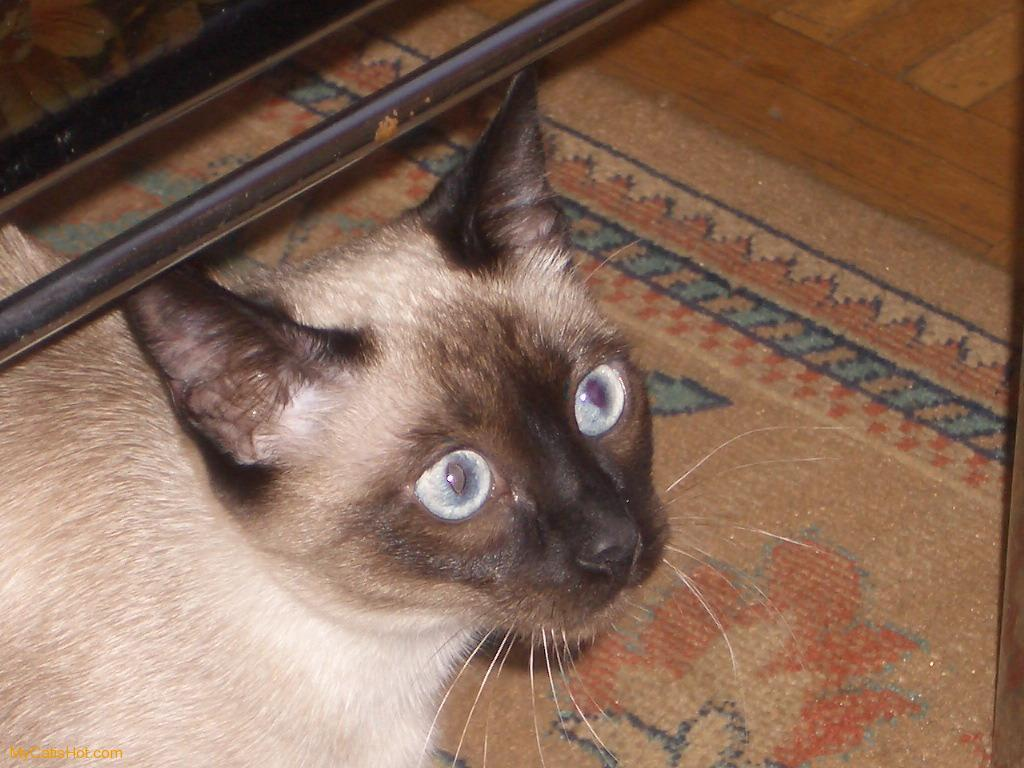
\includegraphics[width=.1\textwidth]{Images/Method/input.jpg}};
	\node[above] at (input.north) {Input image $\vx$};
	\node[draw, trap] (res0) at (-3.5,0) {\rotatebox{90}{\parbox{1.0cm}{\centering{Res-0}}}};
	\node[draw, trap] (res1) at (-1.5,0) {\rotatebox{90}{\parbox{1.0cm}{\centering{Res-1}}}};
	\node[draw, trap] (res2) at (0.5,0) {\rotatebox{90}{\parbox{1.0cm}{\centering{Res-2}}}};
	\node[draw, trap] (res3) at (2.5,0) {\rotatebox{90}{\parbox{1.0cm}{\centering{Res-3}}}};
	\node[draw, trap] (res4) at (4.5,0) {\rotatebox{90}{\parbox{1.0cm}{\centering{Res-4}}}};
	\node[](empt1) at (6.75, 0){};
	\node[draw, rotate=90, align=center] (class) at (7.5,0) {Classifier};
	\node(logit) at (8.25, 0) {$\vy$};
	%%% CLS stream
	\node[](clsin) at (-4, -1.5) {{$\vq_0$}};
	\node[draw](CA0) at (-2.5, -1.5) {{CA-0}};
	\node[draw](CA1) at (-0.5, -1.5) {{CA-1}};
	\node[draw](CA2) at (1.5, -1.5)  {{CA-2}};
	\node[draw](CA3) at (3.5, -1.5)  {{CA-3}};
	\node[draw](CA4) at (5.5, -1.5)  {{CA-4}};

	%% CNN backbone
	\node(empt0) at (-4.65, 0) {};
	\draw[->] (empt0.center) -- node {} (res0);
	\draw[->] (res0) -- node[above] {$F_0$} (res1);
	\draw[->] (res1) -- node[above] {$F_1$} (res2);
	\draw[->] (res2) -- node[above] {$F_2$} (res3);
	\draw[->] (res3) -- node[above] {$F_3$} (res4);
	\draw[->, blue, dashed] (res4) -- node {\blue{\normalsize//}} (class);
	\node[](GAP) at (6.25,0.25) {\blue{$\gap$}};
	\draw[->] (class) -- node {} (logit);
	%% CLS Stream
	\draw[->] (clsin) -- node {} (CA0);
	\draw[dashed, ->] (res0.north) -|node {} (CA0);
	\draw[->] (CA0) -- node[above] {$\vq_1$} (CA1);
	\draw[dashed, ->] (res1.north) -|node {} (CA1);
	\draw[->] (CA1) -- node[above] {$\vq_2$} (CA2);
	\draw[dashed, ->] (res2.north) -|node {} (CA2);
	\draw[->] (CA2) -- node[above] {$\vq_3$} (CA3);
	\draw[dashed, ->] (res3.north) -|node {} (CA3);
	\draw[->] (CA3) -- node[above] {$\vq_4$} (CA4);
	\draw[dashed, ->] (res4.north) -|node[above] {$F_4$} (CA4);
	\draw[-] (CA4.east) -| node[right] {$\vq_5$} (empt1.center);
	\draw[->] (empt1.center) -- node {} (class);
\end{tikzpicture}
\vspace{3pt}
\caption{\emph{\OURS (\Ours) applied to ResNet-based architectures.} Given a network $f$, we replace global average pooling (\gap) by a learned, attention-based pooling mechanism implemented as a stream in parallel to $f$. The feature tensor $F_\ell \in \real^{p_\ell \times d_\ell}$ (\emph{key}) obtained by stage Res-$\ell$ of $f$ interacts with a \cls token (\emph{query}) embedding $\vq_\ell \in \real^{d_\ell}$ in block CA-$\ell$, which contains cross attention~\eq{CA} followed by a linear projection~\eq{qk-layer} to adapt to the dimension of $F_{\ell+1}$. Here, $p_\ell$ is the number of patches (spatial resolution) and $d_\ell$ the embedding dimension. The query is initialized by a learnable parameter $\vq_0 \in \real^{d_0}$, while the output $\vq_5$ of the last cross attention block is used as a global image representation into the classifier. The network and classifier are pretrained and kept frozen while the parameters of \Ours are learned. At inference, we use existing post-hoc interpretability methods like Grad-CAM~\citep{DBLP:journals/corr/SelvarajuDVCPB16} to obtain saliency maps for both the baseline \gap and our \Ours. We compare interpretability metrics as well as accuracy.}
\label{fig:fig_method}
\end{figure*}

%------------------------------------------------------------------------------


\paragraph{Training}

In this sense, the network $f$ is pretrained and remains frozen while we learn the parameters of our \Ours on the same training set as one used to train $f$. The classifier is kept frozen too. Referring to~\eq{f-decomp}, $f_0, \dots, f_L$ and $g$ are fixed, while \gap is replaced by learned weighted averaging, with the weights obtained by the \Ours.

\paragraph{Inference}

As it stands, \Ours is not an interpretability method, but rather a modification of the baseline architecture, \ie, an attention-based pooling mechanism that replaces \gap to enhance the contribution of relevant image regions in the prediction. We are interested in investigating the interpretability properties of this modification. We therefore employ existing post-hoc, CAM-based interpretability methods to generate saliency maps with both baseline \gap and \Ours. We then compare interpretability metrics as well as classification accuracy.

